\chapter{Аналіз поточних досягнень}
\label{sec:analys}

Оскільки область, охоплена темою даної роботи є достатньо широкою, то аналіз доступних можливостей можна розділити на декілька частин:

\begin{itemize}
  \item співставлення зображень, не пов'язане з ключовими точками;
  \item пошук ключових точок та визначення їх дескрипторів;
  \item пошук відповідностей між знайденими ключовими точками;
  \item використання отриманих відповідностей для подальших цілей.
\end{itemize}

\section{Співставлення без ключових точок}
\label{sec:non-keypoint}

Людству відомо багато методів розпізнавання об'єктів на зображеннях. В кожному з них можна виділити переваги та недоліки, однак є деякі характеристики, що об'єднують всі підходи:

\begin{itemize}
  \item для пошуку використовується деяка вихідна інформація, наприклад еталонні зображення;
  \item кожне нове зображення шуканого об'єкту не може абсолютно точно співпадати з еталонними. Вони можуть відрізнятися: 
    \begin{itemize}
      \item змінами в освітленості, або кольорі;
      \item змінами в напрямі та куті огляду;
      \item змінами форми та розмірів;
    \end{itemize}
  \item наперед не можливо задати всі можливі вигляди об'єктів.
\end{itemize}

Взагалі, наукою запропоновано багато видів особливостей зображень, на базі яких можна створювати системи їх співставлення, наприклад: пошук контурів та границь об'єктів~\cite{Mikolajczyk03shape}, розгляд багатовимірних гістограм~\cite{Schiele00recognitionwithout}, що описують розподіл вимірів на частинах зображення. Інші властивості, що можна включити в розгляд при аналізі зображень, включають: колір, рух, опис регіонів зображень. 
Нижче наведено основні напрями досліджень розпізнавання об'єктів, що не пов'язані з відшуканням ключових точок.

\subsection{Визначення границь}

Визначення границь є одним із фундаментальних інструментів в апараті обробки зображень, особливо в задачах визначення особливостей зображень. Метою визначення границь на зображенні є пошук точок зображення, в яких присутня різка зміна яскравості, або, формально - розриви.

Метою визначення границь на зображенні є можливість визначення важливих подій та змін у середовищі, зображеному на рисунку. Можна показати, що за деяких припущень, щодо шляху отримання зображення, розриви в яскравості зображення, зазвичай, відповідають:

\begin{itemize}
  \item змінам глибини;
  \item змінам орієнтації поверхні;
  \item змінам властивостей матеріалів;
  \item змінам в освітленні сцени.
\end{itemize}

\begin{figure}[h]
  \begin{minipage}[h]{0.49\linewidth}
    \includegraphics[width=\linewidth]{detal}
  \end{minipage}
  \hfill
  \begin{minipage}[h]{0.49\linewidth}
    \includegraphics[width=\linewidth]{detal_edges}
  \end{minipage}
  \caption{Приклад відшукання границь зображення за допомогою детектора Кані.}
  \label{fig:canny_edges}
\end{figure}

В ідеальному випадку, результатом використання механізму визначення границь (детектора) є набір замкнутих кривих, що показують границі об'єктів та границі, що відповідають розривам в орієнтаціях поверхонь об'єктів, як наприклад, на рис.~\ref{fig:canny_edges}. 

\subsubsection{Детектор Кані}

Оператор визначення границь Кані~\cite{Canny:1986:CAE:11274.11275} був розроблений Джоном Ф. Кані у 1986 році, і використовує багатокроковий алгоритм для визначення границь зображень. Основними цілями, які Кані ставив при розробці алгоритму були:

\begin{itemize}
  \item хороша ефективність: алгоритм має відшукувати якнайбільше границь на зображенні;
  \item добра локалізація: відмічені границі мають бути якнайближче до реальних границь в зображенні;
  \item стійкість результату: знайдені границі на зображенні мають бути позначені лише раз, і, за можливістю, шум зображення не має створювати додаткових границь.
\end{itemize}

Алгоритм Кані знаходження границь зображення складається з наступних кроків: 

\begin{enumerate}
  \item Подолання шуму. Для цього Кані використовує першу похідну гаусіана. Отже, першим кроком є згортка вихідного зображення з гаусівським фільтром, результатом якої є дещо замилене зображення, що позбавлене точкового шуму. Наприклад для розміру вікна $5\times5$ гаусівський фільтр для $\sigma=1.4$ буде мати вигляд:

\begin{equation}
  B=\frac{1}{159} 
  \begin{bmatrix}
    2 & 4  & 5  & 4  & 2 \\
    4 & 9  & 12 & 9  & 4 \\
    5 & 12 & 15 & 12 & 5 \\
    4 & 9  & 12 & 9  & 4 \\
    2 & 4  & 5  & 4  & 2 \\
  \end{bmatrix}
  \ast A.
\end{equation}

Приклад застосування такої фільтрації до деякого зображення приведено на рис~\ref{fig:castle-smooth}.

\begin{figure}[h]
  \begin{minipage}[h]{0.49\linewidth}
    \includegraphics[width=\linewidth]{castle_025_noisy}
  \end{minipage}
  \hfill
  \begin{minipage}[h]{0.49\linewidth}
    \includegraphics[width=\linewidth]{castle_025_noisy_smooth}
  \end{minipage}
  \caption{Приклад подолання шуму зображення за допомогою гаусівської фільтрації з вікном $5\times5$.}
  \label{fig:castle-smooth}
\end{figure}

  \item Відшукання градієнтів інтенсивності зображення. Оскільки границі на зображенні можуть мати безліч різних напрямів, то алгоритм Кані використовує чотири фільтри для визначення горизонтальних, вертикальних та діагональних границь на зображенні. Оператор визначення градієнту зображення (наприклад оператор Собеля) дає на виході значення першої похідної в горизонтальному ($G_y$) та вертикальному ($G_x$) напрямах, з яких можна визначити розмір та напрям градієнту яскравості розмитого зображення як:
    \begin{align}
      G = \sqrt{G_x^2 + G_y^2} \\
      \Theta = arctan(\frac{G_y}{G_x})
    \end{align}
    Напрямки градієнтів округлюються до одного з чотирьох кутів, що відповідають вертикальному, горизонтальному та двом діагональним напрямам (наприклад 0$\degree$, 45$\degree$, 90$\degree$, 135$\degree$).
  \item Далі позбавляються від не екстремальних точок. Для цього, за допомогою оцінки градієнтів зображення, шукають точки, що є локальними максимумами в напрямку градієнту. Наприклад:
    \begin{itemize}
      \item якщо округлений кут градієнту рівний $0\degree$ (тобто границя має північно-південній напрямок) точка вважається макисимумом, якщо розмір градієнту в цій точці більший за розміри градієнту у східному та західному напрямках;
      \item для кута рівного $45\degree$ (північно-західний - південно-східний напрям), точка вважається границею, якщо її інтенсивність перевищує інтенсивності в північно-східному на південно-західному напрямах;
      \item і т. д.
    \end{itemize}
  \item Подвійна порогова фільтрація. Використання порогової фільтрації допомагає уточнити, чи дійсно присутня границя в поточній точці зображення. Чим менший поріг, тим більше границь потрапить до результату, але результат стане менш стійким до шуму. З іншого боку, високий поріг може проігнорувати слабкі границі, або отримати границі фрагментами. У детекторі Кані використовується фільтрація з двома порогами: якщо значення в точці зображення перевищує верхній поріг, то точка вважається достовірною границею. Інакше, якщо значення менше нижнього порогу, то точка відкидаєтсья. Точки, що лежать між двома порогами вважаються ймовірними кандидатами. Рішення, щодо них виноситься на наступному кроці.
  \item Трасування областей невизначеності. Застосовується до точок, що потрапили до зони невизначеності на попередньому кроці. Вважається, що точка є границею, якщо хоча б один з її восьми сусідів є достовірною границею, і відкидається, інакше. 
\end{enumerate}

\subsection{Кольорові гістограми}

Колір зображуваного об'єкта зумовлений двома фізичними факторами:

\begin{enumerate}
  \item Спектральним розподілом випромінювання.
  \item Відбивною здатністю поверхні об'єкта.
\end{enumerate}

В обробці зображень, зазвичай, використовується кольоровий простір RGB (red, green, blue). Тим не менш, простір RGB не є таким, що сприймається рівномірно, тобто різниця між кольорами в просторі RGB, не відповідає різниці, що сприймається людиною~\cite{Paschos2001}. Крім того, координати RGB є високо корельованими. На відміну від RGB, L*u*v* та L*a*b* є чуттєво-рівномірними, а HSV (Hue, Saturation, Value - відтінок, насиченість, яскравість) є приблизно рівномірним. Тим не менш, ці кольорові простори є чутливими до шуму. В результаті немає остаточної думки щодо того, який з них є найефективнішим, тому на практиці зустрічається цілий набір кольорових просторів.

Представивши інформацію про кольори зображуваних об'єктів в одному з наведених вище просторів, можна побудувати гістограми розподілу значень як сукупності всіх каналів зображення, так і кожного окремо. 

Гістограми розподілу кольорів, зазвичай мають подібний розподіл для одних і тих самих об'єктів, але відрізняються для різних.

Приклад побудови кольорової гістограми наведено на рис~\ref{fig:color-hist}.

\coolfigure{jump_hist}{Приклад побудови кольорових гістограм для деякого фото-зображення}{fig:color-hist}

\section{Ключові точки та дескриптори}

Часто поняття ключових точок та ``кутів'' зображення використовують як синоніми для опису точкових особливостей зображення, що має двомірну структуру. Назва ``кут'' з'явилася за часів перших алгоритмів, що проводили пошук границь зображення, а потім аналізували їх для пошуку змін у напрямах границь (кутів). Було розроблено алгоритми, що зняли необхідність явного пошуку кутів, наприклад аналізуючи високі рівні кривизни градієнту зображення. Було помічено, що так звані ``кути'' були також знайдені на частинах зображення, що не були кутам в традиційному сенсі (наприклад, детекторами кутів знаходилися світлі плями на темному тлі). Ці точки часто називають точками інтересу, але традиційно використовується термін ``кути''.

\subsection{Детектор кутів Моравіца}

Детектор~\cite{Moravec_1981_1849} Моравіца є одним із перших одних із перших алгоритмів пошуку кутів, і визначає кут, як точку з низькою само-подібністю.

Алгоритм перевіряє кожен піксель зображення, чи присутній на ньому кут, порівнюючи, наскільки клаптик з центром в цьому пікселі, подібний до сусідніх - клаптиків, що є трохи зсунути відносно вихідного. Подібність вимірюється як сума квадратів різниць між двома клаптиками. Менші значення індикують подібність.

Якщо піксель знаходиться в частині з рівномірною яскравістю, то сусідні клаптики будуть виглядати подібними. Якщо піксель лежить на границі, то сусідні клаптики, що лежать в напрямку перпендикулярному границі, будуть суттєво відрізнятися, але ті, що лежать в напрямку, паралельному границі будуть відрізнятися не суттєво. Якщо піксель лежить у зоні зі зміною інтенсивності в усіх напрямках, то жоден з сусідніх клаптиків не буде виглядати подібним.

Сила кута визначається найменшою сумою квадратів різниць між клаптиком та його сусідами (горизонтальними, вертикальними та діагональними). Якщо це число локально максимальне, то це означає, що присутня цікава точка.

\subsection{Детектор Гаріса та Сетфенсена}

Гаріс та Стефенс~\cite{Harris88alvey} удосконалили детектор Моравіца, напряму враховуючи диференціал сили кута відносно напрямку, замість використання зсунутих клаптиків. 

Не втрачаючи загальності, розглядається двовимірне зображення у відтінках сірого. Назвемо його $I$. Розглянемо клаптик зображення, розміром $(u,v)$ та його зсув на $(x,y)$. Зважена сума квадратів різниць між цими клаптиками, позначена $S$, обчислюється як:

\begin{equation}
  S(x,y) = \sum_u \sum_v w(u,v) \, \left( I(u+x,v+y) - I(u,v)\right)^2 .
\end{equation}

$I(u + x,v + y)$ може бути апроксимоване розкладанням в ряд Тейлора. Нехай $I_x$ та $I_y$ - часткові похідні $I$ так, що:

\begin{equation}
  I(u+x,v+y) \approx I(u,v) + I_x(u,v)x+I_y(u,v)y .
\end{equation}

Маємо наближення:

\begin{equation}
  S(x,y) \approx \sum_u \sum_v w(u,v) \, \left( I_x(u,v)x + I_y(u,v)y \right)^2, 
\end{equation}

що може бути переписане у матричній формі:
    
\begin{equation}
  S(x,y) \approx 
  \begin{pmatrix} 
    x & y 
  \end{pmatrix} 
  A 
  \begin{pmatrix} 
    x \\ y 
  \end{pmatrix}, 
\end{equation}

де $A$ - структурний тензор:
    
\begin{equation}
  A = \sum_u \sum_v w(u,v) 
  \begin{bmatrix}
    I_x^2   & I_x I_y \\
    I_x I_y & I_y^2
  \end{bmatrix}
  = 
  \begin{bmatrix} 
    \langle I_x^2 \rangle   & \langle I_x I_y \rangle \\
    \langle I_x I_y \rangle & \langle I_y^2 \rangle 
  \end{bmatrix}
\end{equation}

Ця матриця називається матрицею Гаріса, а кутові дужки позначають усереднення (тобто суму по $(u,v)$).

Кут, або цікава точка, характеризується великою зміною $S$ у всіх напрямках вектора
$\begin{pmatrix} x & y \end{pmatrix}$. Аналізуючи власні числа $A$, ця характеристика може бути виражена наступним чином: $A$ має мати два ``великих'' власних числа для цікавої точки. В залежності від розміру власних чисел, можна зробити наступні висновки:
  \begin{enumerate}
    \item Якщо $\lambda_1 \approx 0$ та $\lambda_2 \approx 0$ тоді цей піксель $(x,y)$ не має цікавих точок.
    \item Якщо $\lambda_1 \approx 0$, а $\lambda_2$ - деяке велике позитивне число, то знайдено границю.
    \item Якщо $\lambda_1$ та $\lambda_2$ - великі, додатні числа, то знайдено кут.
  \end{enumerate}

  Гаріс та Стефенс зазначають, що точне обчислення власних чисел є операцією, що вимагає багато ресурсів, оскільки потребує відшукання квадратного кореню, і тому пропонують наступну функцію $M_c$, де $\kappa$ - параметр настройки чутливості:

\begin{equation}
  M_c = \lambda_1 \lambda_2 - \kappa \, (\lambda_1 + \lambda_2)^2 = \operatorname{det}(A) - \kappa \, \operatorname{trace}^2(A) 
\end{equation}

  Таким чином, алгоритму насправді не є має обчислювати власні числа матриці $A$, а достатньо обчислити її визначник та слід для знаходження кутів, а точніше цікавих точок загалом.

\subsection{SIFT}
\label{sec:sift}

Алгоритм \textbf{SIFT} був вперше запропонований Ловом\cite{Lowe2004}. З того часу він зазнав багатьох модифікацій та вдосконалень. Метод SIFT дозволяє знаходити набір особливостей зображень, інваріантних відносно позиції, повороту та масштабування, що дозволяє проводити співставлення з великою кількістю еталонних зображень та забезпечує стійкість до широкого спектру афінних спотворень, змін 3D точки зору, змін в рівні шуму, освітленості. Особливості є досить розрідженими, тобто кожна особливість може бути співставлена з високою ймовірністю з великою базою даних особливостей з різних зображень. Обчислювальна складність визначення особливостей зменшена за рахунок використання підходу каскаду фільтрів, в якому найбільш складні операції застосовуються лише для частин зображення, що проходять початкові тести. Отримання набору особливостей конкретного зображення складається з наступних кроків:

\begin{enumerate}

\item \textbf{Визначення екстремумів в масштабно-просторовому представленні}: перша частина обчислень проводить пошук по всім можливим масштабам та позиціям зображення. Ця операція ефективно реалізована за допомогою функції гаусівської різниці для визначення потенційних критичних точок, інваріантно, відносно масштабу та орієнтації.

\item \textbf{Локалізація ключових точок}: в кожній потенційній позиції застосовується детальна модель для визначення позиції та масштабу. Ключові точки вибираються за мірою їх стійкості.

\item \textbf{Визначення орієнтації}: одна, або більше орієнтацій визначається для кожної ключової точки, в залежності від напрямів локальних градієнтів зображення. Усі наступні перетворення виконуються відносно до визначених орієнтації, масштабу та позиції для кожної особливості зображення, надаючи інваріантність відносно цих перетворень.

\item \textbf{Дескриптор ключової точки}: при вибраному масштабі розглядаються локальні градієнти зображення навколо кожної ключової точки. Вони перетворюються до вигляду, що враховує значні локальні спотворення контурів та освітлення.

\end{enumerate}

Цей підхід було названо Інваріантним відносно Масштабу Перетворенням Особливостей (Scale Invariant Features Transform, SIFT), оскільки він перетворює дані зображення в маcштабо-незалежні координати, відносно локальних особливостей.

\subsubsection{Визначення екстремумів в масштабно-просторовому представленні}
\label{sec:sift scale space extrema}

Як було зазначено вище, першим етапом роботи вказаного алгоритму є визначення положення та масштабу точок, що будуть досліджуватись на наступних етапах. Для цього необхідно знайти ключові особливості зображення, що є стійкими до зміни масштабу та орієнтації об'єкту. Це досягається пошуком по всіх можливих масштабах, використовуючи неперервну функцію для зменшення масштабу~\cite{Witkin83}. 

Кьондерінком~\cite{Koenderink84} та Ліндебергом~\cite{Lindeberg94scale-spacetheory} було показано, що за умов деяких очевидних припущень, єдиним допустимим масштабно-просторовим ядром є гаусівська функція, тому масштабно-просторовим виглядом зображення є функція $L(x, y, \sigma)$, отримана в результаті згортки гаусівської функції змінного масштабу $G(x,y,\sigma)$ з вихідним зображенням $I(x,y)$:

\begin{equation}
  L(x,y,\sigma) = G(x,y,\sigma) \ast I(x,y),
\end{equation}

де $\ast$ - оператор згортки по $x$ та $y$, а

\begin{equation}
  G(x,y,\sigma) = \frac{1}{2\pi\sigma^2}e^{-(x^2+y^2)/2\sigma^2}.
\end{equation}

Для ефективного визначення стійких ключових точок було запропоновано~\cite{Lowe99objectrec} використовувати масштабно-просторові екстремуми згортки різниці гаусівських функцій з зображенням $D(x,y,\sigma)$, що отримано з різниці двох сусідніх масштабів, що відрізняються сталим коефіцієнтом $k$:

\begin{align}
  \label{eq:dog-scale}
    D(x,y,\sigma) & = (G(x,y,k\sigma) - G(x,y,\sigma)) \ast I(x,y) \notag\\
                  & = L(x,y,k\sigma) - L(x,y,\sigma).
\end{align}

\coolfigure{dog}{Схема побудови масштабно-просторової моделі зображення}{fig:dog}

Емпірично було досліджено~\cite{Lowe2004}, що найкращі результати досягаються для $k=\sqrt2$.

Ефективний підхід до побудови $D(x,y,\sigma)$ зображено на рисунку~\ref{fig:dog}. Вихідне зображення поступово згортається з гаусівськими функціями для отримання зображень з масштабного простору, що відрізняються масштабом в $k$ разів (зліва). Далі, кожна октава масштабного простору (тобто проміжок, границі якого відрізняються вдвічі) ділиться на $s$ інтервалів, тоді $k = 2^{1/s}$. Після цього, з використанням гаусівського фільтра, ми отримуємо $s+3$ зображення для першої октави. З них ми отримаємо значення $D(x,y,\sigma)$ для $s+2$ масштабів: на $s$ шукатимемо екстремум та $2$ --- для граничних умов. Далі, зображення наступної октави можемо отримати, вибравши кожний другий піксель з відповідного зображення попередньої октави.

\coolwfigure{ss_extr}{Кожна точка вибірки порівнюється з її 26 сусідами для пошуку локальних екстремумів}{fig:ss-extr}{0.5\linewidth}

Для визначення локальних екстремумів функції $D(x,y,\sigma)$ кожна точка вибірки порівнюється з 8 сусідніми точками на цьому ж зображенні та по 9 сусідів на наступних більшому та меншому масштабі (рис~\ref{fig:ss-extr}).

\subsubsection{Уточнення позицій ключових точок}

Точність знаходження екстремумів може бути збільшена, за допомогою використання розкладання в ряд Тейлора до другого порядку~\cite{Brown02invariantfeatures}:

\begin{equation}
  \label{eq:d-taylor}
  D(\mathbf{x}) = D + {\frac{\partial D}{\partial \mathbf{x}}}^T \mathbf{x} + \frac12 \mathbf{x}^T \frac{\partial ^2 D}{\partial\mathbf{x}^2}\mathbf{x}
\end{equation}

Звідки можна оцінити $\hat{\mathbf{x}}$:

\begin{equation}
  \label{eq:extr-est}
  \hat{\mathbf{x}} = -\left(\frac{\partial^2 D}{\partial \mathbf{x}^2}\right)^{-1} \frac{\partial D}{\partial \mathbf{x}}
\end{equation}

де $D$ та всі відповідні похідні визначаються в досліджуваній точці вибірки, а $\mathbf{x} = (x,y,\sigma)^T$. Якщо відхилення в будь-якому напрямку виявляється більшим за $0.5$, то досліджувану точку змінюють сусідньою та проводять уточнення заново. Після визначення $\hat{\mathbf{x}}$, його значення додають до досліджуваної точки вибірки. Це і є знайдена точка локального екстремуму. 

Підставивши (\ref{eq:extr-est}) в (\ref{eq:d-taylor}), отримаємо значення $D(\hat{\mathbf{x}})$:

\begin{equation*}
  D(\hat{\mathbf{x}}) = D + \frac12 {\frac{\partial D}{\partial x}}^T \hat{\mathbf{x}}
\end{equation*}

Що в подальшому може бути використано для відкидання точок з низькою контрастністю.

\subsubsection{Визначення орієнтації}

Відшукавши адекватну орієнтацію для кожної ключової точки, базуючись на локальних властивостях зображення, її дескриптор може бути описаним відносно цієї орієнтації, тобто досягнемо інваріантне представлення, відносно повороту зображення.

Для пошуку локальних орієнтацій використовується розмите зображення $L$, що відповідає найближчому масштабу. Це забезпечує інваріантість всіх обчислень відносно масштабування. Для кожної точки, $L(x,y)$, спочатку підраховуються значення довжини градієнту, $m(x,y)$, та орієнтації, $\theta(x,y)$, за допомогою піксельних різниць:

\begin{equation}
  m(x,y) = \sqrt{(L(x+1, y) - L(x-1, y))^2 + (L(x,y+1) - L(x,y-1))^2} 
\end{equation}

\begin{equation}
  \theta(x,y) = \tan^{-1}((L(x,y+1) - L(x,y-1)) / (L(x+1,y) - L(x-1,y)))
\end{equation}

З орієнтацій сусідніх точок створюють гістограму орієнтацій. Для цього вибирають точки з квадрату $16\times16$~\cite{Meng_implementingthe} навколо досліджуваної, та складають з них гістограму, попередньо зваживши їх значення довжиною градієнта та гаусівським вікном з $\sigma$, що в 1.5 перевищує поточний масштаб ключової точки. Кількість елементів гістограми обмежують 36-ма, що покриває всю $360^\circ$ область можливих напрямів.

Піки на гістограмі орієнтацій відповідають домінантним напрямам локальних градієнтів. Для наступних обчислень використовують найбільший пік та напрями, значення яких вище за 80\% найвищого піку. Кожен з обчислених піків інтерполюють за допомогою параболи через 3 сусідні значення. В подальшому кожній з отриманих орієнтацій ставиться у відповідність окремі ключові точки з однаковою позицією на площині зображення та в масштабному просторі. 

\begin{figure}[h]
  \begin{minipage}[h]{0.49\linewidth}
    \center{\includegraphics[width=0.5\linewidth]{sift-local-gradients} \\
    Довжини і напрямки локальних градієнтів у кожній точці в квадратній області навколо досліджуваної. Вони зважуються гаусівським вікном, що позначене синім колом.
    }
  \end{minipage}
  \hfill
  \begin{minipage}[h]{0.49\linewidth}
    \center{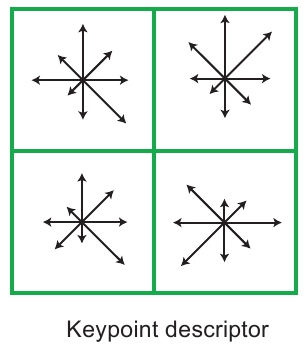
\includegraphics[width=0.5\linewidth]{sift-keypoint-descriptor} \\
    Значення локальних градієнтів з областей $4\times4$ збираються в гістограми з 8-и елементів. Довжини стрілок відповідають сумі довжин локальних градієнтів, близьких за напрямом, в рамках відповідної області.
    }
  \end{minipage}
  \caption{Побудова SIFT-дескрипторів.}
  \label{fig:sift-descriptor}
\end{figure}

\subsubsection{Побудова дескрипторів}

Задачею цього етапу є побудова дескрипторів, що максимально відрізняли б кожну ключову точку. Для цього використовуються довжини та напрями градієнтів навколо досліджуваної ключової точки. Ці значення зображені у вигляді маленьких стрілок у відповідних клітинках на рис~\ref{fig:sift-descriptor}.

На правій частині рис.~\ref{fig:sift-descriptor} зображено отриманий дескриптор ключової точки. На рисунку зображено масив $2\times2$ гістограм орієнтації в той час, як на практиці раціонально використовувати масиви розміром $4\times4$ з 8 значеннями орієнтацій в кожному. Тоді кожній ключовій точці буде відповідати вектор з $4\times4\times8=128$ координатами. 

Кінцевим кроком можна нормалізувати вектори до одиничної довжини, що зменшить вплив зміни контрастності зображення.

Після отримання дескрипторів для всіх ключових точок кожного з досліджуваних зображень, перевірити наявність об'єктів з одних зображень на інших можна за допомогою порівняння (наприклад в евклідовій метриці) значень векторів ключових особливостей кожного із зображень. 

\begin{figure}[h]
  \begin{minipage}[h]{0.49\linewidth}
    \center{
    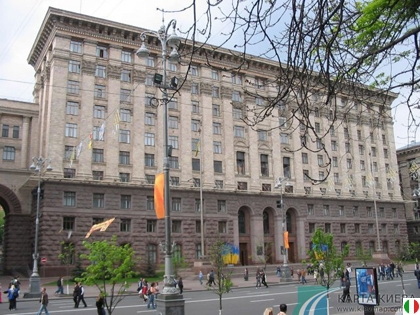
\includegraphics[width=\linewidth]{meria-vhod} \\
    \includegraphics[width=\linewidth]{meria-arka} \\
    }
  \end{minipage}
  \hfill
  \begin{minipage}[h]{0.49\linewidth}
    \center{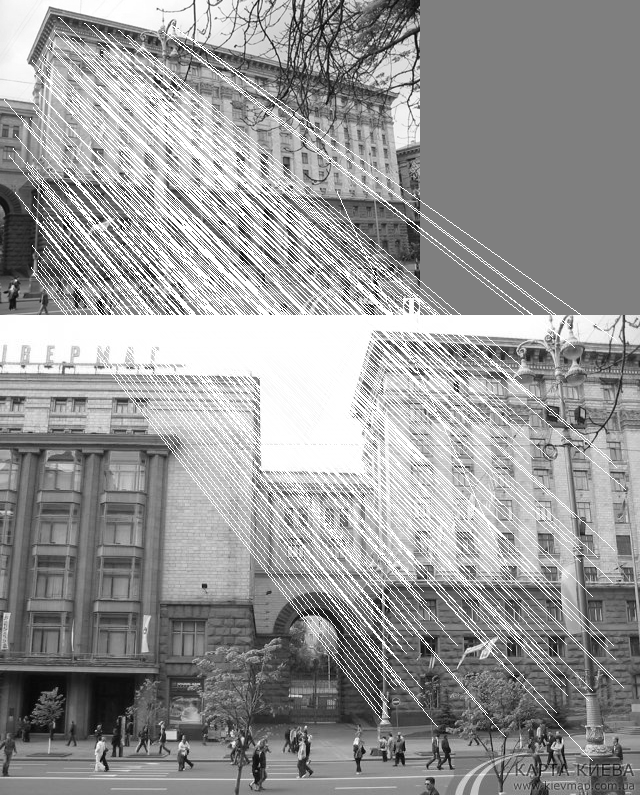
\includegraphics[width=\linewidth]{sift-out} \\
    }
  \end{minipage}
  %\caption{Побудова SIFT-дескрипторів}
  \label{fig:sift-sample}
  \caption{Приклад порівняння зображень за допомогою SIFT.}
\end{figure}

Приклад порівняння двох зображень приведено на рис.~\ref{fig:sift-sample}.

\subsection{ASIFT}
\label{sec:asift}

Якщо об'єкт на зображенні має чіткі, неперервні границі, то його зображення, отримане камерами з різних позицій та кутів огляду, може суттєво змінюватися. Ці трансформації легко наближати афінними перетвореннями площини зображення.

Тим не менш, проблема співставлення різних зображень одного об'єкта, отриманих під різними кутами нахилу, залишається і до нині. Одним з підходів вирішення цієї проблеми може бути побудова дескрипторів для кожної ключової точки зображення, інваріантних відносно афінних перетворень, але таких алгоритмів на сьогоднішній день не існує. 

Алгоритм ASIFT~\cite{Morel2009} (Affine-SIFT) використовує інший підхід. Замість побудови афінно-інваріантних дескрипторів напряму, автором було запропоновано симулювати різні можливі кути нахилу спостерігача (камери) у двох площинах. Так, варіюючи довготу та широту положення камери до вихідного зображення, ми маємо ширші можливості для порівняння двох зображень, що відрізняються кутом огляду, без значного збільшення складності обчислень. Дворозмірна схема роботи ASIFT дозволяє отримати результати, загалом, кращі, ніж SIFT, ускладнюючи обчислення не більше, ніж в два рази. 

Для опису алгоритму використовується нове поняття, \textit{відносний нахил} (\textit{transition tilt}), що описує рівень спотворення зображення при переході від одного кута огляду до іншого. 

\subsubsection{Модель отримання вихідного зображення}
Робота алгоритму ASIFT базується на наступній моделі отримання цифрового зображення (рис~\ref{fig:camera-model}).

\coolwfigure{camera-model}{Модель цифрової камери: $\textbf{u}=\textbf{S}_1G_1\mathcal{A}u_0$. $\mathcal{A}$ - перетворення плоскої проекції (гомографія). $G_1$ - згладжуючий гаусівський фільтр. $\textbf{S}_1$ - вибірка CCD матрицею.}{fig:camera-model}{0.5\linewidth}

Як зображено на рис~\ref{fig:camera-model}, отримання зображення плоского об'єкту може бути описане наступним чином:

\begin{equation}
  \textbf{u}=\textbf{S}_1G_1A\mathcal{T}u_0
\end{equation}

де $\textbf{u}$ -- отримане цифрове зображення, а $u_0$ - нескінченний фронтальний вигляд плоского об'єкта. $\mathcal{T}$ та $A$ -- відповідно зміщення та плоска проекція, пов'язані з переміщенням камери. $G_1$ -- гаусівська згортка, що моделює оптичне розмиття, а $\textbf{S}_1$ -- оператор дискретизації зображення на сітці з кроком 1. 

Далі, апроксимують оператор $A$, що насправді дає зображення в перспективі, афінним перетворенням для спрощення обчислень. Тим не менш дана апроксимація є досить точною, оскільки в подальшому розглядають лише локальні особливості зображення, а при розгляданні малих його областей перспектива майже повністю співпадає з плоским афінним перетворенням. Також аналогічний результат видно з розкладання будь-якого неперервного перетворення в ряд Тейлора. В кожній точці перетворення може бути описано афінним оператором. Таким чином, всі локальні ефекти перспективи можуть бути змодельовані як $u(x,y) \rightarrow u(ax+by+e, cx+dy+f)$ в кожній точці.

Морелом було доведено~\cite{Morel2009} наступну теорему. 

\textsc{Теорема.}
\textit{
Будь-який лінійний оператор 
$A=\begin{bmatrix}a&b \\ c&d\end{bmatrix}$ з $detA > 0$, що не є тотожною матрицею може бути представлений єдиним чином у вигляді розкладу:
  \begin{equation}
    \label{eq:asift-decomposition}
    A = H_\lambda R_1(\psi)T_tR_2(\phi) =     
    \lambda \begin{bmatrix} 
      \cos \psi & -\sin\psi \\
      \sin\psi  & \cos\psi
    \end{bmatrix}
    \begin{bmatrix}
      t & 0 \\
      0 & 1 
    \end{bmatrix}
    \begin{bmatrix} 
      \cos \phi & -\sin\phi \\
      \sin\phi  & \cos\phi
    \end{bmatrix}
  \end{equation}
  де $\lambda>0$, $\lambda t$ - визначник матриці $A$, $R_i$ - повороти, $\phi \in \left[0,\pi\right)$, та $T_t$ - нахил, що є діагональною матрицею з власними числами $t>1$ та 1.
}

Отриманий результат є пов'язаним з принципом SVD-розкладу. 

\coolwfigure{asift-decomposition}{Геометрична інтерпретація розкладу~\ref{eq:asift-decomposition}.}{fig:asift-decomposition}{0.2\linewidth}

На рисунку~\ref{fig:asift-decomposition} зображено графічну інтерпретацію наведеного вище розкладу. $\phi$ та $\theta= \arccos1/t$ - кути огляду, $\psi$ параметризує обертання камери, а $\lambda$ відповідає масштабу. Площина, що містить нормаль і оптичну вісь, утворює кут $\phi$ з деякою фіксованою вертикальною площиною. Цей кут називають довготою. Оптична вісь утворює з нормаллю кут $\theta$, який називають широтою. 

\subsubsection{Відносний нахил}

Параметр $t$ в \ref{eq:asift-decomposition} називається \textit{абсолютним нахилом}, оскільки описує відхилення фактичної точки зору від фронтального вигляду. Для виміру спотворень між двома зображеннями, що відрізняються кутом нахилу, також вводять поняття \textit{відносного нахилу}.

\textsc{Означення}. Розглянемо два вигляди плоского зображення, $u_1(x,y) = u(A(x,y))$ та $u_2(x,y)=u(B(x,y))$ де $A$ та $B$ -- два такі оператори, що $BA^{-1} \ne I$. Використовуючи позначення з \ref{eq:asift-decomposition}, будемо називати відповідно \textit{відносним нахилом} $\tau(u_1,u_2)$ та \textit{відносним поворотом} $\psi(u_1,u_2)$ єдині значення параметрів такі, що 
\[
  BA^{-1} = H_\lambda R_1(\phi)T_\tau R_2(\psi).
\]

\subsubsection{Алгоритм ASIFT}
\label{sec:algo-asift}
Алгоритм ASIFT складається з наступних кроків:

\begin{enumerate}
    \item Для кожного з вхідних зображень симулюються всі можливі спотворення, викликані відхиленням оптичної осі камери від фронтального положення. Ці спотворення описуються двома параметрами: довготою $\psi$ та широтою $\phi$. Після обертання на кут $\phi$, зображення нахиляють з параметром $t = \left| \frac{1}{\cos\theta}\right|$ (нахил на $t$ в напрямку $x$ є операцією $u(x,y) \rightarrow u(tx,y)$). Для цифрових зображень поворот реалізується направленим $t$-сабсемплінгом і вимагає попереднього згладжування згорткою з гаусівською функцією з дисперсією $c\sqrt{t^2-1}$. Значення $c=0.8$ було вибрано Ловом~\cite{Lowe2004}.
    \item Ці повороти і нахили проводяться для скінченної і невеликої кількості кутів довготи і широти. При цьому кроки дискретизації для цих параметрів вибираються так, щоб для кожного можливого значення цих параметрів поблизу знаходилася точка отриманої сітки дискретизації.
    \item Всі отримані симуляцією зображення порівнюються за допомогою деякого іншого алгоритму (SIFT).
\end{enumerate}

\coolwfigure{asift-sampling}{Дискретизація параметрів $\theta=\arccos 1/t$ та $\phi$. Зліва: зображення в перспективі півкулі спостережень (показані лише $t=2,2\sqrt{2},4$). Справа: вигляд з зеніту півсфери спостереження.}{fig:asift-sampling}{0.8\linewidth}

Дискретизація параметрів спотворення проводиться наступним чином:
\begin{itemize}
  \item широта $\theta$ вибирається так, що відповідні нахили утворюються геометричну прогресію $1, a, a^2, \ldots,a^n$, з $a>1$. Значення $a = \sqrt{2}$ є добрим компромісом між точністю і розрідженістю;
  \item довгота $\phi$ для кожного значення нахилу утворює арифметичну прогресію $0, b/t, \ldots, kb/t$, де значення $b \simeq 72^{\degree}$ також є раціональним компромісом, а $k$ -- найбільше ціле число таке, що $kb/t < 180^{\degree}$.
\end{itemize}


\subsubsection{Оптимізація двома розмірами}

Для прискорення роботи алгоритму ASIFT, використовується схема роботи з зображеннями двох розмірів. Спочатку, алгоритм, описаний в \ref{sec:algo-asift}, застосовують до зменшених варіантів досліджуваних зображень. У випадку успішного співставлення малих зображень, процедура вибирає отримані значення афінного перетворення та, застосовуючи їх до повнорозмірних зображень, порівнює їх за допомогою алгоритму SIFT. Дворозмірний метод можна описати наступними кроками:

\begin{enumerate}
  \item Зменшення досліджуваного та еталонного зображення в K$\times$K разів: $\mathbf{u}' = \mathbf{S}_K\mathbf{G}_K\mathbf{u}$ та $\mathbf{v}' = \mathbf{S}_K\mathbf{G}_K\mathbf{v}$, де $\mathbf{G}_K$ -- згладжуючий гаусівський дискретний фільтр, а $\textbf{S}_K$ -- оператор зменшення розміру зображення (subsampling) в K$\times$K разів
  \item Застосування алгоритму ASIFT, описаного в \ref{sec:algo-asift}, до зменшених зображень $u'$ та $v'$.
  \item Вибрати $M$ афінних перетворень, що дають найбільшу кількість збігів на зменшених зображеннях $u'$ та $v'$.
  \item Застосувати ASIFT до  $u$ та $v$, але симулювати лише $M$ афінних перетворень.
\end{enumerate}

\section{Пошук відповідностей між ключовими точками}
\label{sec:keypoints}
Наступною задачею, після обчислення значень дескрипторів для знайдених ключових точок, є пошук відповідностей між знайденими точками. Оскільки кожен дескриптор є числовим вектором у деякому багатовимірному просторі, то для цього можна використовувати наявні алгоритми вирішення цієї задачі. 

Як показує досвід, пошук відповідностей є процесом, на який витрачається найбільша кількість часу та ресурсів у задачах комп'ютерного зору. До сьогодні не відомо точного алгоритму для пошуку найближчих сусідів, швидшого за лінійний. Тим не менш, було показано~\cite{muja_flann_2009}, що наближені алгоритми здатні забезпечити суттєве прискорення роботи з лише невеликими втратами у точності результатів. Варто зазначити, що для вирішення конкретної задачі співставлення точок зображення, ми можемо використати додаткову інформацію про походження даних багатовимірних векторів. Оскільки очікується, що на досліджуваних зображеннях зображено одні і ті ж об'єкти, то можна очікувати, що взаємне розміщення точок на двох порівнюваних зображеннях буде приблизно однаковим. В рамках даної роботи, під час вибору методу, що найкраще відповідав би поставленій задачу було розглянуто наступні підходи:

\begin{itemize}
  \item \textbf{виснажливий пошук} серед всіх можливих варіантів. Полягає в переборі всіх заданих пар векторів багатовимірного простору та відшуканні відстані, між елементами кожної з них з наступим вибором пар, що відповідають найменшим відстаням. Цей підхід було відкинуто, через високі вимоги до обчислювальних ресурсів та незадовільний час роботи, що унеможливлює його застосування, наприклад, в системах реального часу. Крім того, він показав низку стійкість до ``викидів'', тобто точок, що отримали схожі дескриптори, але насправді відповідають різним частинам досліджуваних об'єктів;
  \item \textbf{швидкий пошук приблизних найближчих сусідів}~\cite{muja_flann_2009} (англ. FLANN - Fast Approximate Nearest Neighbours with Automatic Algorithm Configuration) - показав значно кращі результати по швидкодії в порівнянні з виснажливим пошуком. Тим не менш, було також відкинуто, оскільки він не враховує особливості даних, що розглядаються;
  \item \textbf{RANSAC}. Цей алгоритм позбавлений недоліків попередніх двох, оскільки він успішно виконує обидві поставлені задачі: шукає наближений результат за допомогою випадкових вибірок та здатен врахувати особливості даних, до яких він застосовується.
\end{itemize}

\subsection{RANSAC}
\label{sec:ransac}

RANSAC (англ. Random Sample Consensus) - підхід, запропонований Фішлером та Боллесом~\cite{Fischler:1981:RSC:358669.358692}, що використовується для оцінки параметрів математичних моделей за допомогою набору даних, що включає випадкові викиди. Цей алгоритм не є детермінованим, тобто надає результат, що може вважатися вірним з деякою заданою ймовірністю, хоча цю ймовірність можна збільшувати зі збільшенням кількості ітерацій. 

Робота алгоритму базується на припущенні, що весь набір даних складається з двох частин: ``добрі точки'', розподіл яких описується деякими параметрами заданої моделі та ``викидів'' - даних, що погано описуються моделлю. Крім того, викиди можуть бути спричинені зашумленістю даних. 

На вході алгоритм отримує наступні дані: набір значень вхідних та вихідних спостережуваних величин, параметризовану модель, що може пояснити, або апроксимувати спостереження та деякі параметри точності оцінювання. Результат отримують за допомогою ітеративного вибору підмножини з вихідних даних. На цій підмножині будується та оцінюється гіпотеза наступним чином:

\begin{enumerate}
    \item Шукають модель, що найкраще описує вибрану підмножину гіпотетичних ``добрих точок'', тобто обчислються всі параметри моделі.
    \item Оцінюється степінь відповідності моделі всім іншим точкам вихідних даних, і, якщо точка відповідає моделі, то вона також додається до множини ``хороших''.
    \item Вважається, що гіпотетична модель є достатньо доброю, якщо багато точок були успішно описані цією моделлю. 
    \item Модель переоцінюється з використанням всіх гіпотетичних вдалих точок.
    \item Оцінюється помилка моделі, щодо точок, що були нею успішно описані. 
\end{enumerate}

Тут параметрами точності алгоритму є значення максимальної нев'язки між змодельованим вихідним значенням та спостережуваним для того, щоб включити точку до множини успішних та частка вхідних даних, що має бути успішно описана моделлю, щоб можна було вважати її прийнятною.

Перевагою даного алгоритму є те, що він дозволяє використати додаткову інформацію про природу вихідних даних, яку можна описати структурою моделі, параметри якої підбираються алгоритмом. 

Оскільки можна показати\cite{Szeliski:2005fk}, що геометричне перетворення точок між зображеннями одного і того ж плоского об'єкта з різних точок зору може бути описане проективним перетворенням, яке в свою чергу можна задати матрицею \ref{eq:homography} розмірності $3\times3$ так, що:

  \begin{equation}
    \label{eq:homography}
    p_a = 
    \begin{bmatrix}
      x_a  \\
      y_a  \\
      1
    \end{bmatrix}
    ,
    p^\prime_b = 
    \begin{bmatrix} 
      w^{\prime}x_b \\
      w^{\prime}y_{b} \\
      w^{\prime}
    \end{bmatrix}
    , 
    \mathbf{H}_{ab} = 
    \begin{bmatrix} 
      h_{11} & h_{12} & h_{13} \\
      h_{21} & h_{22} & h_{23} \\
      h_{31} & h_{32} & h_{33} 
    \end{bmatrix} 
    ,
  \end{equation}

тоді

  \begin{equation*}
    p^\prime_b = \mathbf{H}_{ab}p_a
  \end{equation*}
   та
  \begin{equation*}
    p_b = p^\prime_b/w^\prime = 
    \begin{bmatrix} 
      x_b  \\
      y_b  \\
      1
    \end{bmatrix}.
  \end{equation*}

Таким чином, цю інформацію можна використати для побудови оцінюваної моделі для співставлення точок в алгоритмі RANSAC, тобто оцінити параметри матриці проективного перетворення, використовуючи для оцінки гіпотез алгоритму RANSAC нев'язку між спостережуваними значеннями точок та отриманими за допомогою гіпотетичної моделі. 

\coolfigure{ransac_homo}{Приклад співставлення ключових точок за допомогою алгоритму RANSAC. Малими кругами зображені ключові точки. Лініями позначені відповідності між точками двох зображень. Зелені лінії відповідають точкам, зв'язок між якими добре описується моделлю.}{fig:ransac}

Отриманої на даному кроці інформації уже може бути достатньо для деяких попередніх висновків щодо об'єктів, зображених на досліджуваних зображеннях, наприклад про наявність, кількість об'єктів, що цікавлять дослідника, тощо. Приклад роботи алгоритму RANSAC зображено на рис.~\ref{fig:ransac}

\section{Висновки до розділу \ref{sec:analys}}

В розділі було проаналізовано як деякі історичні, так і найновітніші алгоритми, що знаходять застосування при вирішення задач порівняння зображень, серед яких: пошук границь на зображеннях за допомогою детектора Кані, порівняння кольорових гістограм, детектори кутів Моравіца, Гаріса та Стефенсена, алгоритми SIFT, ASIFT та RANSAC.

Було показано, що при вирішенні задачі розпізнавання об'єктів на зображеннях, що можуть бути отримані різними камерами при різних обставинах, таких як: різні рівні освітленості, положення об'єктів та камер відносно сцени та відносно одне одного, доцільно використовувати саме підходи до співставлення зображень, що базуються на локальних особливостях.

Серед відповідного класу алгоритмів, призначених для пошуку та опису локальних особливостей, в якості об'єкту подальшого дослідження, що полягає в аналізі поведінки та результатів роботи алгоритму при обробці відеопотоків, було вибрано: ASIFT - найбільш ефективний із широко відомих на сьогоднішній день, SURF та SIFT.

Оскільки історично склалося, що дані алгоритми було розроблено з думкою про обробку статичних зображень, то це надає суттєвий потенціал для подальшого їх розвитку, зокрема покращень їх ефективності за рахунок додаткової інформації, що не доступна при обробці статичних зображень.
